\documentclass[10pt,onecolumn,twoside,letterpaper]{article}
\usepackage[text={7.7in,9.5in},centering]{geometry}
\usepackage[spanish,es-nodecimaldot]{babel}

\usepackage{hyperref}

\usepackage{multicol}
\usepackage{wrapfig}

\usepackage{amsmath,amssymb,amsthm}

\usepackage{harvard}% bibliographystyle: apsr, agsm, dcu, kluwer, nederlands
\newcommand{\myreferences}{../../../doc/review/review/library}
\usepackage{graphicx}
\graphicspath{{../../../doc/images/}}
\usepackage{amssymb}
\usepackage{fancyhdr}
\usepackage{color}
\usepackage{colortbl}
\definecolor{gray}{cmyk}{0.0,0.0,0.0,0.60}

\usepackage{float}

\usepackage{mcode}

%\usepackage{auto-pst-pdf}
%\usepackage{pst-all}

%\usepackage[numbered]{mcode}
%\usepackage{lipsum}

\pagestyle{fancy}
\fancyhf{}
\fancyhead[RO]{\small{\textcolor{gray}{\textsc{Hacia un framework de locomoci\'on b\'ipeda, evolutiva y flexible}}}}
\fancyhead[LO]{
\includegraphics[scale=0.05]{unlogo.png}}
\fancyhead[LE]{
\includegraphics[scale=0.05]{unlogo.png}\quad\small{\textcolor{gray}{\textsc{Control Inteligente 2015-01}}}}
\fancyhead[RE]{\small{\textcolor{gray}{\textsc{TALLER 02}}}}
\fancyfoot[CO,CE]{\thepage}
\fancyfoot[LO,RE]{\scriptsize{\textcolor{gray}{\emph{Version 0.2}}}}

\title{\vspace{-0.8cm}
\includegraphics[scale=0.12]{unescudobn.png}\\\vspace{-0.0cm}
  \LARGE \textbf{Taller 2 - Fundamentos de L\'ogica y Conjutos Difusos}}
\author{J.A. Castillo-Le\'on\thanks{jacastillol@unal.edu.co} \and Ronny Gelleschus\thanks{rgelleschus@unal.edu.co}}
\date{}

\begin{document}
\maketitle
\begin{abstract}\noindent\small\textit{En el siguiente documento se hacen ejercicios de repaso de los fundamentos b\'asicos de los conjutos difusos y las relaciones difusas. La implicaci\'on es la relaci\'on que mas se detalla. Finalmente un sistema experto de toma de decisiones se construye y analiza con MATLAB.}
\end{abstract}\vspace{1cm}

%\begin{multicols}{2}

\par{\bf \large Punto 1:} Considere el conjuto difuso $\mathcal{C}$, llamado \emph{``aproximadamente uno''}, definido por su funci\'on de pertenencia $\mu_c(x):\mathbb{R}\to[0,1]:$ con $\mu_c=1/(1+(x-1)^2)$. Calcule el $\alpha$-corte de $\mathcal{C}$ para $\alpha=0.5$, $\mathcal{A}_{0.5}$ (ver Figura \ref{fig:Acut05}).\\
Soluci\'on: Como se propone en \cite{Babuska1999}, $\mathcal{A}_{0.5}=\left\{x|\mu_c(x)\geq0.5\right\}$ con $x\in\mathbb{R}$. A continuaci\'on se demuestra que $\mu(x)\,\geq\,0.5\,\forall x \in [0,2]$,
\begin{align*}\small
  \mu_c&=1/(1+(x-1)^2)\geq 0.5 \tag{intercambiando}
  \\0.5&\leq 1/(1+(x-1)^2) \tag{observar que: $1+(x-1)^2\geq 1\,\forall x\in\mathbb{R}$}
  \\0.5(1+(x-1)^2)&\leq 1 \tag{reduciendo}
  \\(x-1)^2-1&\leq 0 \tag{reduciendo}
  \\x(x-2)&\leq 0 
\end{align*}
Notar primero que $x\leq 0\,\forall x\in(-\infty,0]$ y segundo que $(x-2)\leq0\,\forall x\in(-\infty,2]$. Usando el producto de los dos intervalos con la restricci\'on se concluye que $x\in [0,2]$.
\begin{figure}[H]
 \centering
 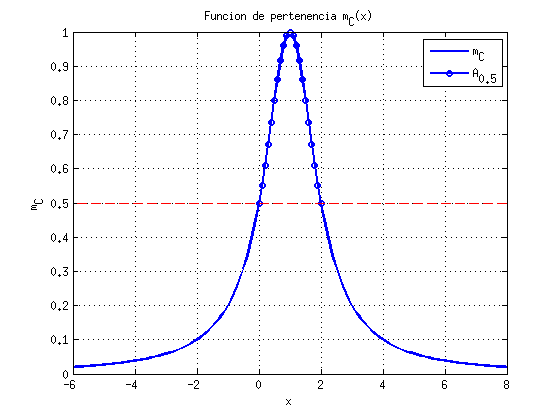
\includegraphics[scale=0.6]{A_05.png}
 \caption{Conjunto $\mathcal{A}_{0.5}$}
 \label{fig:Acut05}
\end{figure}
\par{\bf \large Punto 2:} Considere los conjutos difusos $\mathcal{A}$ y $\mathcal{B}$, tales que el $core(\mathcal{A})\cap core(\mathcal{B})\,=\,\emptyset$
\par{\bf 2.1: ¿Es el conjuto difuso $\mathcal{C}\,=\,\mathcal{A}\cap \mathcal{B}$ normal? Por qu\'e?}\\
Por definici\'on seg\'un \cite{Babuska1999}, $core(\mathcal{A})=\left\{x|\,\mu_A=1\right\}$, $supp(\mathcal{A})=\left\{x|\,\mu_A>0\right\}$ y $\mathcal{A}_{\alpha}=\left\{x|\,\mu_A\geq\alpha\right\}$, por lo tanto al definir los conjutos por comprens\'ion o por propiedad, $\emptyset=core(\mathcal{A})\cap core(\mathcal{B})=\left\{x|\,\mu_A=1\right\}\wedge\left\{x|\,\mu_B=1\right\}=\left\{x|\,\mu_A=1\,\wedge\,\mu_B=1\right\}=core(\mathcal{A}\cap\mathcal{B})$, por lo tanto se puede concluir que $\mathcal{C}$ no es normal.\\
\par{\bf 2.2: ¿Es el conjuto difuso $\mathcal{C}\,=\,\mathcal{A}\cap \mathcal{B}$ convexo o no convexo? Por qu\'e?}\\
El conjunto difuso $\mathcal{C}$ puede ser tanto convexo como no convexo y depende de las caracter\'isticas de $\mathcal{A}$ y $\mathcal{B}$, a continuaci\'on se describen dos ejemplos para soportar la afirmaci\'on anterior, para ello se toma la definici\'on: \emph{Un conjunto difuso} $\mathcal{A}$ \emph{es convexo si} $\forall \alpha\in[0,1]$, \emph{el intervalo de corte} $\mathcal{A}_\alpha$ \emph{es convexo}. De la misma forma, \emph{Un conjunto difuso} $\mathcal{A}$ \emph{es no convexo si} $\exists \alpha\in[0,1]$, \emph{tal que ese intervalo de corte} $\mathcal{A}_\alpha$ \emph{es no convexo}
\par \textcolor{blue}{\texttt{Caso convexo:}} Suponga $\mathcal{A}$ y $\mathcal{B}$ son convexos, por lo tanto $\mathcal{A}\cap\mathcal{B}$ es convexo.
\par \textcolor{blue}{\texttt{Caso no convexo:}} Suponga $\mathcal{A}$ es no convexo tal que $\exists{\alpha}_{nc}|\,(\alpha_{nc}\in(0,1))\wedge(\mathcal{A}_{\alpha_{nc}}\text{ es no convexo})$ y $\mathcal{B}$ es convexo tal que $\mathcal{A}_{\alpha_{nc}}\cap\mathcal{B}_{\alpha_{nc}}\neq\emptyset$ y a su vez es no convexo, por lo tanto $\mathcal{A}\cap\mathcal{B}$ es no convexo.
\begin{figure}[H]
 \centering
 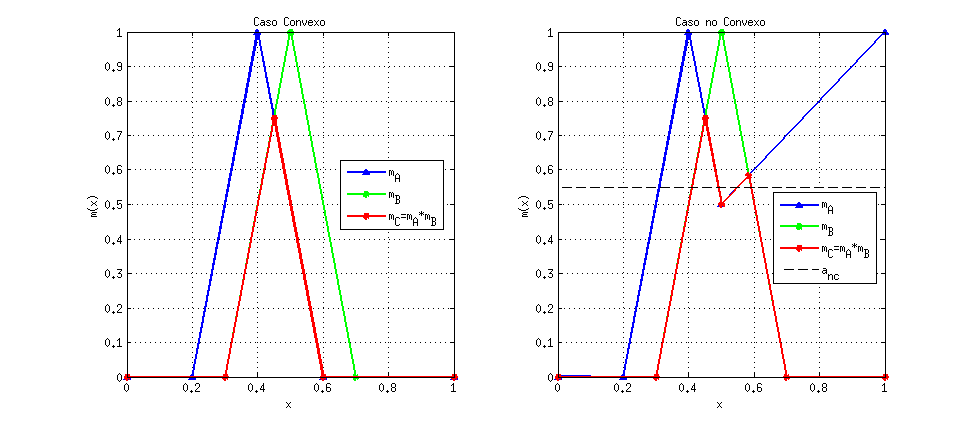
\includegraphics[scale=0.6]{CnvxOrNotCnvx.png}
 \caption{Conjunto convexo $\mathcal{C}$(Izq). Conjunto no convexo $\mathcal{C}$(Der)}
 \label{fig:CnvxOrNotCnvx}
\end{figure}
\par{\bf 2.3: Cardinalidad y condiciones para $card(\mathcal{C})>0$}\\
\par Seg\'un \cite{Babuska1999}, \emph{Cardinalidad de un conjunto difuso finito $\mathcal{A}=\left\{x_1,x_2,\ldots,x_n\right\}$, $card(\mathcal{A})$ como $\left|\mathcal{A}\right|=\sum_{i=1}^n\mu_A(x_i)$}. Se puede decir que si $\mathcal{A}$ es finito y el conjuto cl\'asico $supp(\mathcal{A})\neq\emptyset$ entonces $card(\mathcal{A})>0$. Y al igual si $\mathcal{B}$ es finito y el conjuto cl\'asico $supp(\mathcal{B})\neq\emptyset$ entonces $card(\mathcal{B})>0$, adem\'as si $supp(\mathcal{A})\cap supp(\mathcal{B})\neq\emptyset$ se puede afirmar que por lo anterior $card(\mathcal{C})>0$.
\par{\bf \large Punto 3:} Calcular las proyecciones de $\mathcal{A}$ sobre $X$ y $Y$.
\begin{equation}
  \label{eq:ej3}
  \mathcal{A}\,=\,\left\{0.2/(x_1,y_1),0.3/(x_1,y_2),0.6/(x_2,y_1),0.8/(x_2,y_2)\right\}
\end{equation}
aplicanado la proyecci\'on sobre el eje $X$, $proj_X(\mathcal{A})=\left\{max(\mu_1,\mu_2)/x_1,max(\mu_3,\mu_4)/x_2\right\}$ seg\'un\cite{Babuska1999}, remplazando $proj_X(\mathcal{A})=\left\{max(0.2,0.3)/x_1,max(0.6,0.8)/x_2\right\}$ y simplificando $proj_X(\mathcal{A})=\left\{0.3/x_1,0.8/x_2\right\}$. De la misma manera se opera con el eje $Y$ obteniendo $proj_Y(\mathcal{A})=\left\{0.6/y_1,0.8/y_2\right\}$  (ver Figura \ref{fig:ProyA}.a).
\par{\bf \large Punto 4:} Calcular la extensi\'on cil\'indrica de $\mathcal{A}$ sobre $X\times Y$.
\begin{equation}
  \label{eq:ej3}
  \mathcal{A}\,=\,\left\{0.3/(x_1),0.5/(x_2)\right\}
\end{equation}
aplicanado la extensi\'on cil\'indrica $ext_Y(\mathcal{A})=\left\{0.3/(x_1,y),0.5/(x_2,y)\mid y\in Y\right\}$ (ver Figura \ref{fig:ProyA}.b).
\begin{figure}[H]
 \centering
 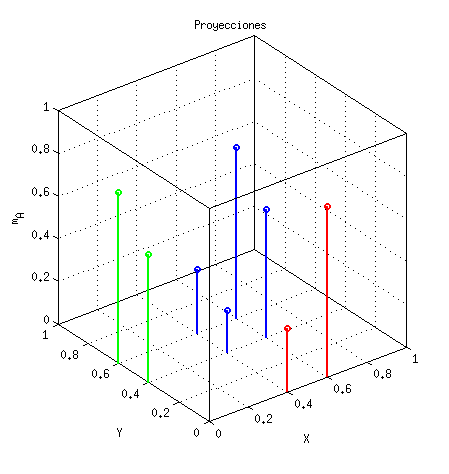
\includegraphics[scale=0.6]{ProjA.png}
 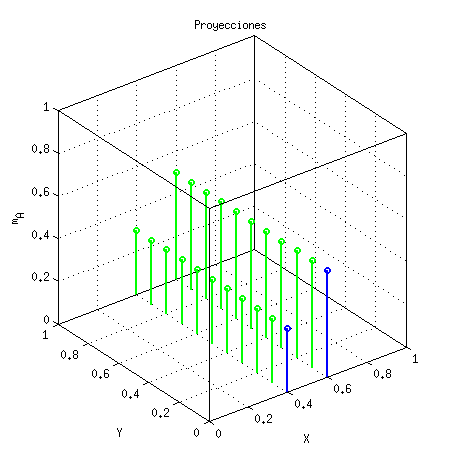
\includegraphics[scale=0.6]{ExtA.png}\\
 a)\hspace{7.5cm}b)
 \caption{a) Proyecci\'on sobe el eje $X$ y sobre el eje $Y$, b) Extensi\'on cilindrica sobre el plano $X\times Y$}
 \label{fig:ProyA}
\end{figure}
\par{\bf \large Punto 5:} Definici\'on de etiqueta ling\"uistica y variable ling\"uistica\\
En un ejemplo cuando se habla de \emph{altura}, se puede definir a la variable ling\"uistica $x$ como la \emph{altura}. Los ``valores'' que puede tomar $x$ est\'an dentro de un conjuto de etiquetas ling\"uistica, como por ejemplo \{\emph{alto, medio, bajo}\}.
\par \textcolor{blue}{\texttt{Etiqueta Ling\"uistica:}} Es una palabra que representa el ``valor'' de una variable, por ejemplo \emph{la temperatura}, toma su ``valor'' de \emph{alto}, a la que se pueden asociar diferentes valores n\'umericos. M\'as espec\'ifico una etiqueta ling\"uistica representa un conjuto difuso caracterizado por una funci\'on de pertenencia o membrec\'ia. Es una forma de discretizar el universo discurso de una variable ling\"uistica $x$ en varios subconjuntos.
\par \textcolor{blue}{\texttt{Variable Ling\"uistica:}} Se puede decir, el conjuto (o uni\'on) que representa a todas las etiquetas ling\"uisticas y reproduce el universo de discurso describe a su vez a la variable ling\"uistica.
\par{\bf \large Punto 6:} Dada una relacion difusa $\mathbf{R}:X\times Y\to[0,1]$:\\
\begin{equation*}
  \label{eq:relation}
  \mathbf{R}\,=\,
  \begin{array}{cccc}
    &y_1&y_2&y_3\\
    x_1&0.7&0.3&0.1\\
    x_2&0.4&0.8&0.2\\
    x_3&0.1&0.2&0.9
  \end{array}
\end{equation*}
y un conjuto difuso $\mathcal{A}\,=\,\left\{0.1/x_1,1/x_2,0.4/x_3\right\}$, determinar $\mathcal{B}\,=\,\mathcal{A}\circ\mathbf{R}$, primero con el operador $max$-$min$ y luego con el operador $max$-$prod$.
\par \textcolor{blue}{\texttt{Operador max-min:}} 
\begin{equation*}
  \label{eq:relation}
  min(ext_Y(\mathcal{A}),\mathbf{R})\,=\,min\left(\left[
  \begin{array}{ccc}
    0.1&0.1&0.1\\
    1.0&1.0&1.0\\
    0.4&0.4&0.4
  \end{array}\right],\left[
  \begin{array}{ccc}
    0.7&0.3&0.1\\
    0.4&0.8&0.2\\
    0.1&0.2&0.9
  \end{array}\right]\right)\,=\,\left[
  \begin{array}{ccc}
    0.1&0.1&0.1\\
    0.4&0.8&0.2\\
    0.1&0.2&0.4
  \end{array}\right]
\end{equation*}
\begin{equation*}
  \label{eq:relmax}
  \mathcal{B}_{min}\,=\,max(min(ext_Y(\mathcal{A}),\mathbf{R}))\,=\,proj_Y\left(min(ext_Y(\mathcal{A}),\mathbf{R})\right)\,=\,\left[0.4,0.8,0.4\right]
\end{equation*}
\par \textcolor{blue}{\texttt{Operador max-prod:}} 
\begin{equation*}
  \label{eq:relation}
  prod(ext_Y(\mathcal{A}),\mathbf{R})\,=\,\left[
  \begin{array}{ccc}
    0.1&0.1&0.1\\
    1.0&1.0&1.0\\
    0.4&0.4&0.4
  \end{array}\right]*\left[
  \begin{array}{ccc}
    0.7&0.3&0.1\\
    0.4&0.8&0.2\\
    0.1&0.2&0.9
  \end{array}\right]\,=\,\left[
  \begin{array}{ccc}
    0.07&    0.03&    0.01\\
    0.4&   0.8&    0.2\\
    0.04&    0.08&    0.36
  \end{array}\right]
\end{equation*}
\begin{equation*}
  \label{eq:relmax}
  \mathcal{B}_*\,=\,max(prod(ext_Y(\mathcal{A}),\mathbf{R}))\,=\,proj_Y(prod\left(ext_Y(\mathcal{A}),\mathbf{R})\right)\,=\,\left[0.4,0.8,0.36\right]
\end{equation*}
$\therefore$ Para todo valor de $y\in Y$ se cumplir\'a siempre que $\mu_{\mathcal{B}_*}(y)\leq \mu_{\mathcal{B}_{min}}(y)$. Los operadores son equivalentes y normalmente la diferencia no ser\'a muy grande. Sin embargo la elecci\'on de un operador u otro cambiar\'a los resultados a la salida. Se podr\'an escoger seg\'un la conveniencia.  
\par{\bf \large Punto 7:} Considerando la  regla $R_i:$ \textbf{if} $x$ is $\mathcal{A}$ \textbf{then} $y$ is $\mathcal{B}$ con conjutos difusos $\mathcal{A}\,=\,\left\{0.1/x_1,0.4/x_2,1.0/x_3\right\}$ y $\mathcal{B}\,=\,\left\{0.0/y_1,1.0/y_2,0.2/y_3\right\}$. Calcule la relaci\'on difusa $\mathbf{R}$ que representa el valor de verdad de esta regla difusa.\\
\par Usando la \emph{t}-norma del m\'inimo,
\begin{equation*}
  \mathbf{R}_M \,=\,\min(ext_Y(\mathcal{A}),ext_X(\mathcal{B}))\,=\,\min\left(\left[
  \begin{array}{ccc}
    0.1&0.1&0.1\\
    0.4&0.4&0.4\\
    1.0&1.0&1.0
  \end{array}\right],\left[
  \begin{array}{ccc}
    0.0&1.0&0.2\\
    0.0&1.0&0.2\\
    0.0&1.0&0.2
  \end{array}\right]\right)\,=\,
\left[
  \begin{array}{ccc}
    0.0&0.1&0.1\\
    0.0&0.4&0.2\\
    0.0&1.0&0.2
  \end{array}
\right]
\end{equation*}
\par Usando la \emph{t}-norma de Lukasiewicz,
\begin{equation*}
  \mathbf{R}_L \,=\,min(1,1-ext_Y(\mathcal{A})+ext_X(\mathcal{B}))\,=\,
\left[
  \begin{array}{ccc}
    0.9&1.0&1.0\\
    0.6&1.0&0.8\\
    0.0&1.0&0.2  
  \end{array}
\right]
\end{equation*}
Al comparar las dos reglas de forma gr\'afica, se observa que siempre se cumple $\mathbf{R}_M\leq\mathbf{R}_L$ (ver Figura \ref{fig:MinVsLuka}). Ademas si se toma, un conjuto arbitrario $\mathcal{A}'\,=\,\left\{0.1/x_1,0.3/x_2,0.1/x_3\right\}$ y se aplica la composici\'on $\mathcal{B}_M\,=\,\mathcal{A}'\circ\mathbf{R}_M$ y $\mathcal{B}_L\,=\,\mathcal{A}'\circ\mathbf{R}_L$, se obtiene $\mathcal{B}_M\,=\,\left\{0.0/y_1,0.4/y_2,0.2/y_3\right\}$ y $\mathcal{B}_L\,=\,\left\{0.6/y_1,1.0/y_2,0.8/y_3\right\}$, se concluye que $\mathcal{B}_M\,\leq\,\mathcal{B}_L$.
\begin{figure}[H]
 \centering
 \includegraphics[scale=0.6]{MinVsLuka.png}
 \caption{Comparaci\'on de la regla $\mathbf{R}_M$ vs $\mathbf{R}_L$}
 \label{fig:MinVsLuka}
\end{figure}
\par{\bf \large Punto 8:} Se considera el sistema de decisi\'on multicriterio para definir la mejor opci\'on laboral. Se consideran como criterios el \emph{salario} $s\in[0,5]M\$$ y la \emph{distancia} $d\in[0,10]km$. Usando las particiones de Ruspini con funciones trapesoidales de pertenencia se usan las siguientes etiquetas ling\"uisticas: $s=\{\mathbf{B}ajo,\mathbf{M}edio,\mathbf{A}lto\}$ y $s=\{\mathbf{P}equena,\mathbf{M}ediana,\mathbf{G}rande\}$. La salida del sistema es la \emph{conveniencia} $c$, con sus respectivas etiquetas $\{\mathbf{I}naceptable,\mathbf{T}olerable,\mathbf{E}xcelente\}$, el universo de discurso se define como $c\in[0,100]\%$\\
\par{\bf 8.1: Funciones de partenencia y base de reglas}\\
En este paso solo se muestran las las funciones de pertenencia hechas por uno de nosotros (\textbf{Jaime Andr\'es}), sin embargo al final se comparan los dos expertos con las \emph{bases de conocimiento} de las reglas de los dos.
\begin{multicols}{2}
  Los par\'ametros de las funciones trapezoidales de los conjutos de pertencia para el \emph{salario} son (ver Figura \ref{fig:UnivS}):
  \begin{lstlisting}
    B = [-0.1,-0.1,0.7,1.3];
    M = [0.7,1.3,3.4,4.0];
    A = [3.4,4.0,5.1,5.1];
  \end{lstlisting}
  \begin{figure}[H]
    \centering
    \hspace{-0.5cm}\includegraphics[scale=0.30]{SalaryUniverse.png}
    \caption{Universo discurso de $s$}
    \label{fig:UnivS}
  \end{figure}
\end{multicols}
\begin{multicols}{2}
  Los par\'ametros de las funciones trapezoidales de los conjutos de pertencia para ls \emph{distancia} son (ver Figura \ref{fig:UnivD}):
  \begin{lstlisting}
    P = [-0.1,-0.1,0.7,1];
    Mn= [0.7,1,3,5];
    G = [3,5,10.1,10.1];
  \end{lstlisting}
  \begin{figure}[H]
    \centering
    \hspace{-0.5cm}\includegraphics[scale=0.3]{DistanceUniverse.png}
    \caption{Universo discurso de $d$}
    \label{fig:UnivD}
  \end{figure}
\end{multicols}
\begin{multicols}{2}
  Los par\'ametros de las funciones trapezoidales de los conjutos de pertencia para la \emph{conveniencia} son (ver Figura \ref{fig:UnivC}):
  \begin{lstlisting}
    I = [-0.1,-0.1,25,40];
    T = [25,40,60,75];
    E = [60,75,100.1,100.1];
  \end{lstlisting}
  \begin{figure}[H]
    \centering
    \hspace{-0.5cm}\includegraphics[scale=0.3]{ConvenienceUniverse.png}
    \caption{Universo discurso de $c$}
    \label{fig:UnivC}
  \end{figure}
\end{multicols}
\begin{multicols}{2}[La base de reglas se representa por el siguiente recuadro (\textbf{Ronny} izquierda y \textbf{Jaime Andr\'es} derecha):]
\begin{lstlisting}
%            Distance  d
%            P   Mn    G
%          ---------------
%  S  B  ||  T |  I |  I |
%  a  M  ||  E |  T |  T |
%  l  A  ||  E |  E |  T |
%          ---------------
\end{lstlisting}
\begin{lstlisting}
%            Distance  d
%            P   Mn    G
%          ---------------
%  S  B  ||  T |  I |  I |
%  a  M  ||  E |  T |  T |
%  l  A  ||  E |  E |  E |
%          ---------------
\end{lstlisting}
\end{multicols}
en donde por ejemplo en la tabla de la izquierda la regla $\mathbf{R}_{2,2}$ : \textbf{If} s es $\mathcal{M}$ \textbf{and} d es $\mathcal{Mn}$ \textbf{then} c es $\mathcal{T}$.\\
\begin{multicols}{2}[A continuaci\'on las 9 reglas:]
\textbf{Ronny}\\
{\small
\par$\mathbf{R}_{1,1}$ : \textbf{If} s es $\mathcal{B}$ \textbf{and} d es $\mathcal{P}$ \textbf{then} c es $\mathcal{T}$\\
\par$\mathbf{R}_{1,2}$ : \textbf{If} s es $\mathcal{B}$ \textbf{and} d es $\mathcal{M}n$ \textbf{then} c es $\mathcal{I}$\\
\par$\mathbf{R}_{1,3}$ : \textbf{If} s es $\mathcal{B}$ \textbf{and} d es $\mathcal{G}$ \textbf{then} c es $\mathcal{I}$\\
\par$\mathbf{R}_{2,1}$ : \textbf{If} s es $\mathcal{M}$ \textbf{and} d es $\mathcal{P}$ \textbf{then} c es $\mathcal{E}$\\
\par$\mathbf{R}_{2,2}$ : \textbf{If} s es $\mathcal{M}$ \textbf{and} d es $\mathcal{M}n$ \textbf{then} c es $\mathcal{T}$\\
\par$\mathbf{R}_{2,3}$ : \textbf{If} s es $\mathcal{M}$ \textbf{and} d es $\mathcal{G}$ \textbf{then} c es $\mathcal{T}$\\
\par$\mathbf{R}_{3,1}$ : \textbf{If} s es $\mathcal{A}$ \textbf{and} d es $\mathcal{P}$ \textbf{then} c es $\mathcal{E}$\\
\par$\mathbf{R}_{3,2}$ : \textbf{If} s es $\mathcal{A}$ \textbf{and} d es $\mathcal{M}n$ \textbf{then} c es $\mathcal{E}$\\
\par$\mathbf{R}_{3,3}$ : \textbf{If} s es $\mathcal{A}$ \textbf{and} d es $\mathcal{G}$ \textbf{then} c es $\mathcal{T}$}\\

\textbf{Jaime Andr\'es}\\
{\small
\par$\mathbf{R}_{1,1}$ : \textbf{If} s es $\mathcal{B}$ \textbf{and} d es $\mathcal{P}$ \textbf{then} c es $\mathcal{T}$\\
\par$\mathbf{R}_{1,2}$ : \textbf{If} s es $\mathcal{B}$ \textbf{and} d es $\mathcal{M}n$ \textbf{then} c es $\mathcal{I}$\\
\par$\mathbf{R}_{1,3}$ : \textbf{If} s es $\mathcal{B}$ \textbf{and} d es $\mathcal{G}$ \textbf{then} c es $\mathcal{I}$\\
\par$\mathbf{R}_{2,1}$ : \textbf{If} s es $\mathcal{M}$ \textbf{and} d es $\mathcal{P}$ \textbf{then} c es $\mathcal{E}$\\
\par$\mathbf{R}_{2,2}$ : \textbf{If} s es $\mathcal{M}$ \textbf{and} d es $\mathcal{M}n$ \textbf{then} c es $\mathcal{T}$\\
\par$\mathbf{R}_{2,3}$ : \textbf{If} s es $\mathcal{M}$ \textbf{and} d es $\mathcal{G}$ \textbf{then} c es $\mathcal{T}$\\
\par$\mathbf{R}_{3,1}$ : \textbf{If} s es $\mathcal{A}$ \textbf{and} d es $\mathcal{P}$ \textbf{then} c es $\mathcal{E}$\\
\par$\mathbf{R}_{3,2}$ : \textbf{If} s es $\mathcal{A}$ \textbf{and} d es $\mathcal{M}n$ \textbf{then} c es $\mathcal{E}$\\
\par$\mathbf{R}_{3,3}$ : \textbf{If} s es $\mathcal{A}$ \textbf{and} d es $\mathcal{G}$ \textbf{then} c es $\mathcal{E}$}\\
\end{multicols}

\par{\bf 8.2: Superficie de decisi\'on}\\
Se obtuvo la superficie:
\begin{figure}[H]
  \centering
  \includegraphics[scale=0.5]{ExpertRG.png}
  \includegraphics[scale=0.5]{ExpertJACK02.png}\\
  a)\hspace{8cm}b)
  \caption{Superficies de decisi\'on de trabajo. a) Sistema experto de \textbf{Ronny}, b) Sistema experto de \textbf{Jaime Andr\'es}}
  \label{fig:SurfDecision}
\end{figure}
\par{\bf Analisis y conclusiones}\\
De las superficies de decisi\'on de la figura \ref{fig:SurfDecision}, se puede ver diferencias, lo siguiente a simple vista:
\begin{itemize}
\item Jaime Andr\'es trabajar\'ia lejos si el salario es alto. 
\item Ronny toma mucho m\'as en cuenta la distancia como factor de conveniencia. A Ronny le gusta caminar.
\item Jaime Andr\'es tiene una mayor \'area de rechazo de empleo.
\end{itemize}
Se prob\'o con 3 casos y se obtuvo lo siguiente:
\par \textcolor{blue}{\texttt{Caso 1:}} Salario de 1.5 millones a una distancia de 3 kilom\'etros de la vivienda. 
\begin{figure}[H]
  \centering
  \textbf{Ronny}\\
  \includegraphics[width=0.9\textwidth]{c15_30RG.png}\\
  \textbf{Jaime Andr\'es}\\
  \includegraphics[width=0.9\textwidth]{c15_30JA.png}\\
  \caption{\small Conjunto de inferencia y defuzificaci\'on en la parte de arriba \textbf{Ronny} 78.45\% y en la grafica de abajo \textbf{Jaime Andr\'es} 50\%}
  \label{fig:UnivC}
\end{figure}
\par \textcolor{blue}{\texttt{Caso 2:}} Salario de 1.9 millones a una distancia de 0.2 kilom\'etros de la vivienda. 
\begin{figure}[H]
  \centering
  \textbf{Ronny}\\
  \includegraphics[width=0.7\textwidth]{c19_02RG.png}\\
  \textbf{Jaime Andr\'es}\\
  \includegraphics[width=0.7\textwidth]{c19_02JA.png}\\
  \caption{\small Conjunto de inferencia y defuzificaci\'on en la parte de arriba \textbf{Ronny} 89.44\% y en la grafica de abajo \textbf{Jaime Andr\'es} 83.72\%}
  \label{fig:UnivC}
\end{figure}
\par \textcolor{blue}{\texttt{Caso 3:}} Salario de 3.9 millones a una distancia de 1.1 kilom\'etros de la vivienda. 
\begin{figure}[H]
  \centering
  \textbf{Ronny}\\
  \includegraphics[width=0.7\textwidth]{c39_11RG.png}\\
  \textbf{Jaime Andr\'es}\\
  \includegraphics[width=0.7\textwidth]{c39_11JA.png}\\
  \caption{\small Conjunto de inferencia y defuzificaci\'on en la parte de arriba \textbf{Ronny} 89.12\% y en la grafica de abajo \textbf{Jaime Andr\'es} 76.5\%}
  \label{fig:UnivC}
\end{figure}

%\end{multicols}

%\nocite{*}
\bibliographystyle{nederlands}% apsr, agsm, dcu, kluwer, nederlands
\bibliography{\myreferences}
\end{document}
